\section{ExplainableCropAI Framework}

This section presents the architecture and components of our proposed ExplainableCropAI framework. We first provide a high-level overview of the system, followed by detailed descriptions of each component and their integration.

\subsection{System Architecture Overview}

ExplainableCropAI is designed as an integrated framework that combines disease detection with multi-level explanations and context-aware recommendations. Figure \ref{fig:system-architecture} illustrates the overall architecture, which consists of five primary components:

\begin{enumerate}
    \item \textbf{Base Disease Detection Model}: A deep learning model for accurate classification of paddy diseases from leaf images
    \item \textbf{Visual Explanation Generator}: Techniques to highlight important regions in the image that influenced the prediction
    \item \textbf{Uncertainty Quantification Module}: Methods to estimate and communicate model confidence
    \item \textbf{Natural Language Explanation Generator}: Domain-specific templates to translate visual evidence into human-readable explanations
    \item \textbf{Recommendation Engine}: Knowledge-based system to provide context-aware treatment and management suggestions
\end{enumerate}

\begin{figure}[ht]
    \centering
    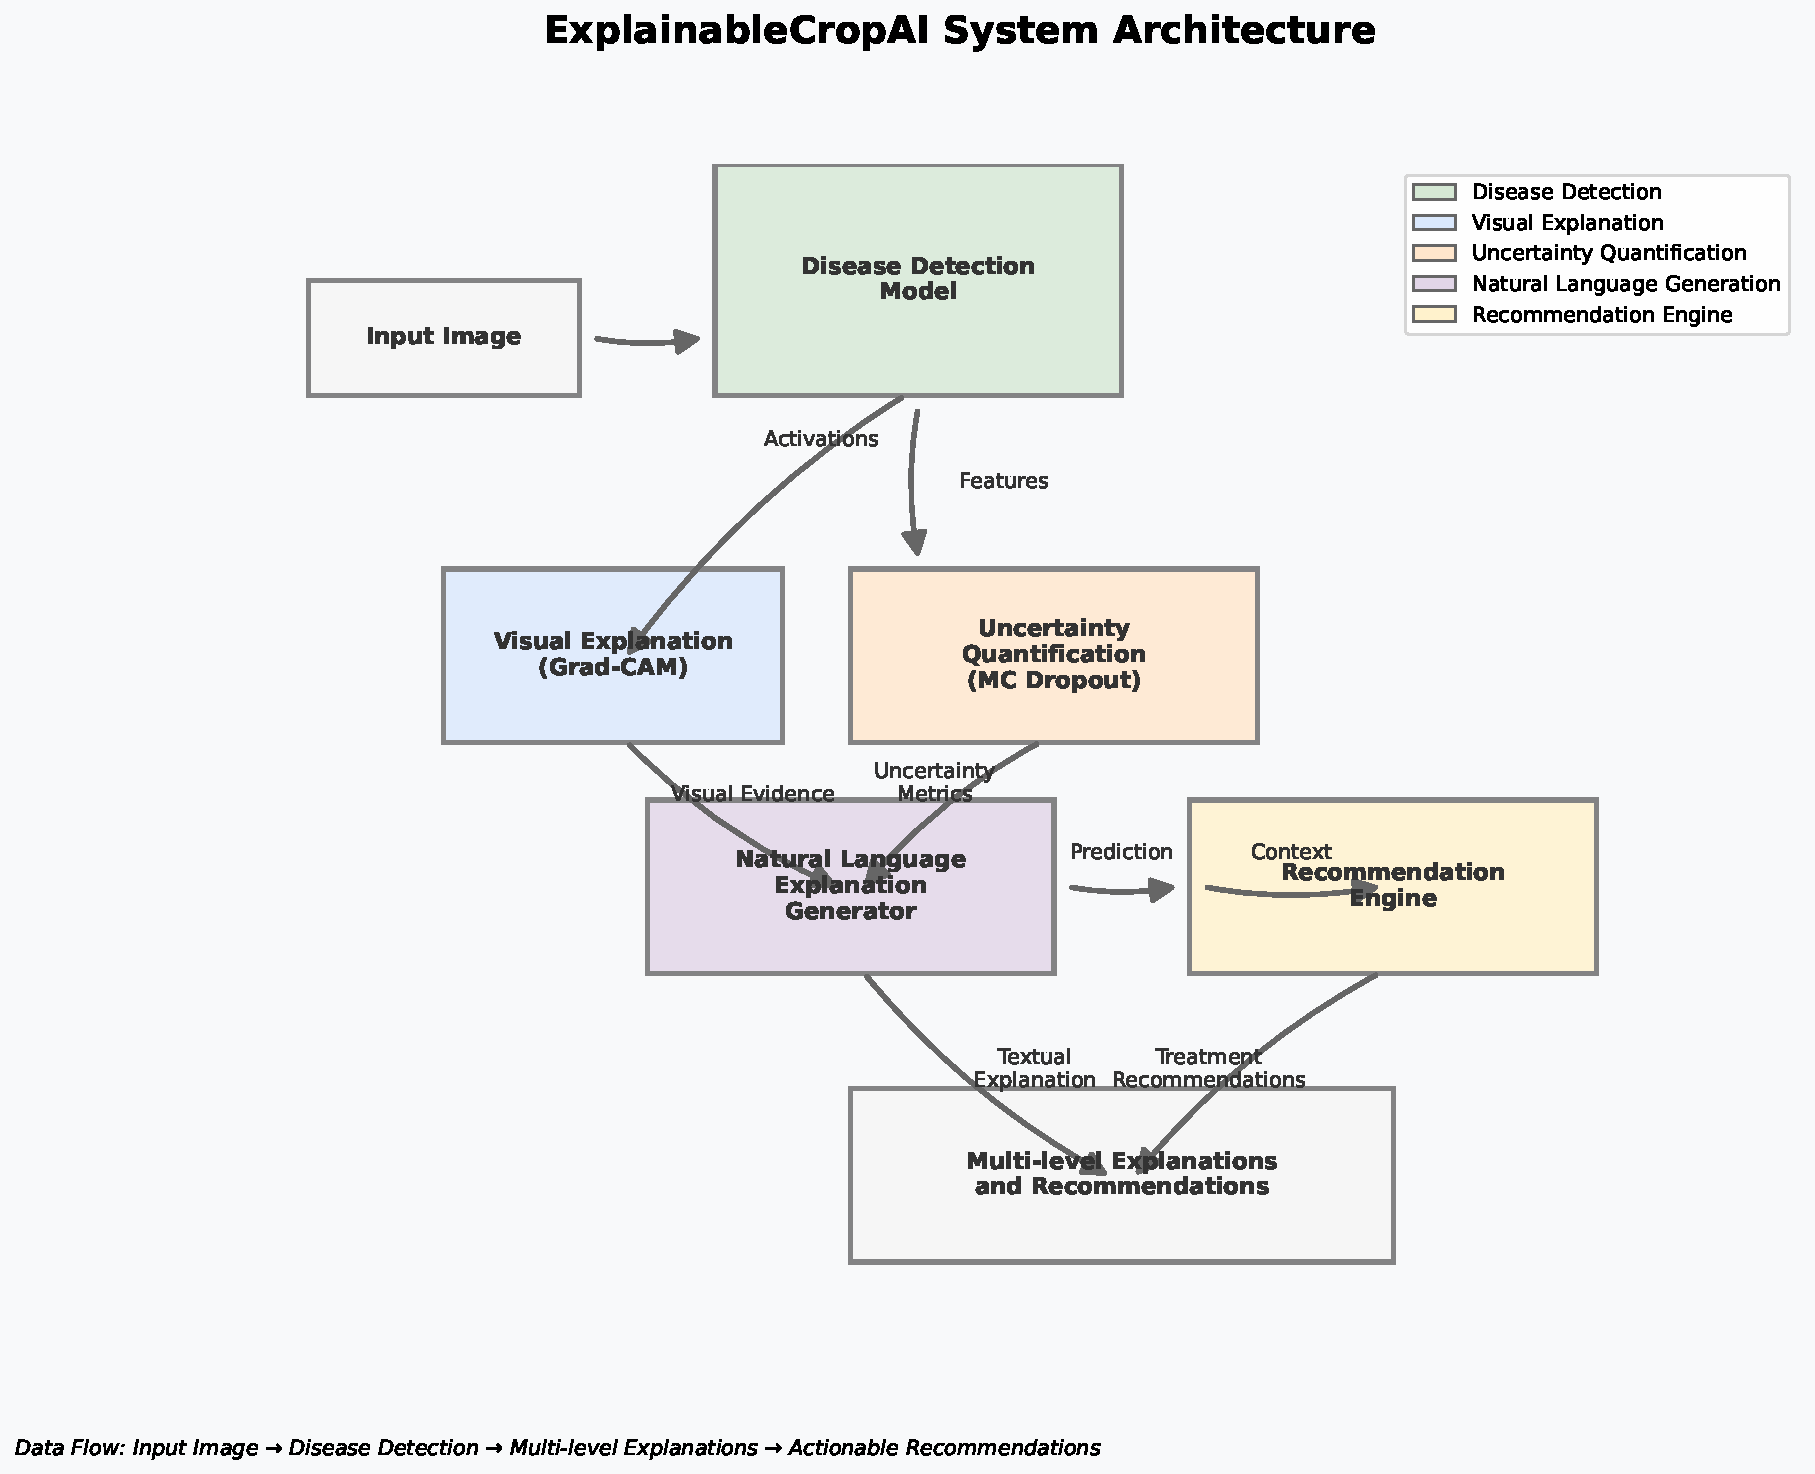
\includegraphics[width=0.9\textwidth]{../results/figures/system_architecture.pdf}
    \caption{ExplainableCropAI system architecture showing the integration of disease detection, multi-level explanations, and recommendation generation.}
    \label{fig:system-architecture}
\end{figure}

The framework operates as follows: An input image is processed by the base disease detection model to generate a prediction. Simultaneously, the model's internal representations are analyzed by the visual explanation generator to identify regions contributing to the prediction. The uncertainty quantification module performs multiple forward passes with dropout to estimate prediction confidence. Visual evidence and uncertainty information are then processed by the natural language explanation generator, which creates a human-readable explanation using domain-specific templates. Finally, the recommendation engine combines the prediction, explanation, and additional contextual information to generate actionable treatment and management suggestions.

\subsection{Base Disease Detection Model}

Our base disease detection model is a convolutional neural network (CNN) that classifies paddy leaf images into one of several disease categories or identifies them as healthy. We selected ResNet50 \cite{he2016deep} as our backbone architecture due to its balance of accuracy and computational efficiency, but with several modifications to facilitate explainability:

\begin{itemize}
    \item We removed the final global average pooling layer and replaced it with a custom pooling mechanism that preserves spatial information
    \item We added hooks to capture gradients and activations at intermediate layers
    \item We incorporated dropout layers not only for regularization but also to enable uncertainty quantification
\end{itemize}

The model was trained on the Paddy Doctor dataset \cite{das2020paddy}, which contains 10,407 images across 10 classes (9 disease categories and healthy). We applied standard data augmentation techniques (random cropping, rotation, flipping, and color jittering) to improve robustness. The model was trained using cross-entropy loss with the Adam optimizer for 100 epochs, employing early stopping based on validation accuracy.

To ensure the model's suitability for deployment in resource-constrained environments, we evaluated inference time on various platforms, including desktop GPUs, mobile devices, and edge computing hardware. The final model achieves 97.5\% accuracy on the test set with an inference time of 125ms on a Nvidia GTX 1080 GPU and 450ms on a Raspberry Pi 4.

\subsection{Multi-level Explanation System}

\subsubsection{Visual Explanations}

Our visual explanation component implements Gradient-weighted Class Activation Mapping (Grad-CAM) \cite{selvaraju2017grad} to generate heatmaps highlighting regions of the image that significantly influenced the model's prediction. Grad-CAM was selected for its class-discriminative properties and computational efficiency compared to alternatives like LIME or SHAP. Figure \ref{fig:gradcam-examples} shows examples of Grad-CAM visualizations for different paddy diseases.

The implementation extracts gradients flowing into the final convolutional layer with respect to the predicted class score. These gradients are global-average-pooled to obtain importance weights for each feature map. The weighted combination of activation maps is then upsampled to the input image resolution and overlaid on the original image, creating an intuitive visualization of regions contributing to the prediction.

To evaluate the quality of visual explanations, we collected a subset of 500 images with pixel-level annotations of disease-affected regions, allowing us to calculate localization metrics such as Intersection over Union (IoU) between explanation heatmaps and ground truth masks.

We conducted user studies to evaluate the interpretability of these visualizations with agricultural stakeholders. Farmers and extension workers found the heatmap overlays intuitive and helpful for verifying that the model was focusing on relevant disease symptoms, increasing their trust in the system's predictions.

\begin{figure}[t]
    \centering
    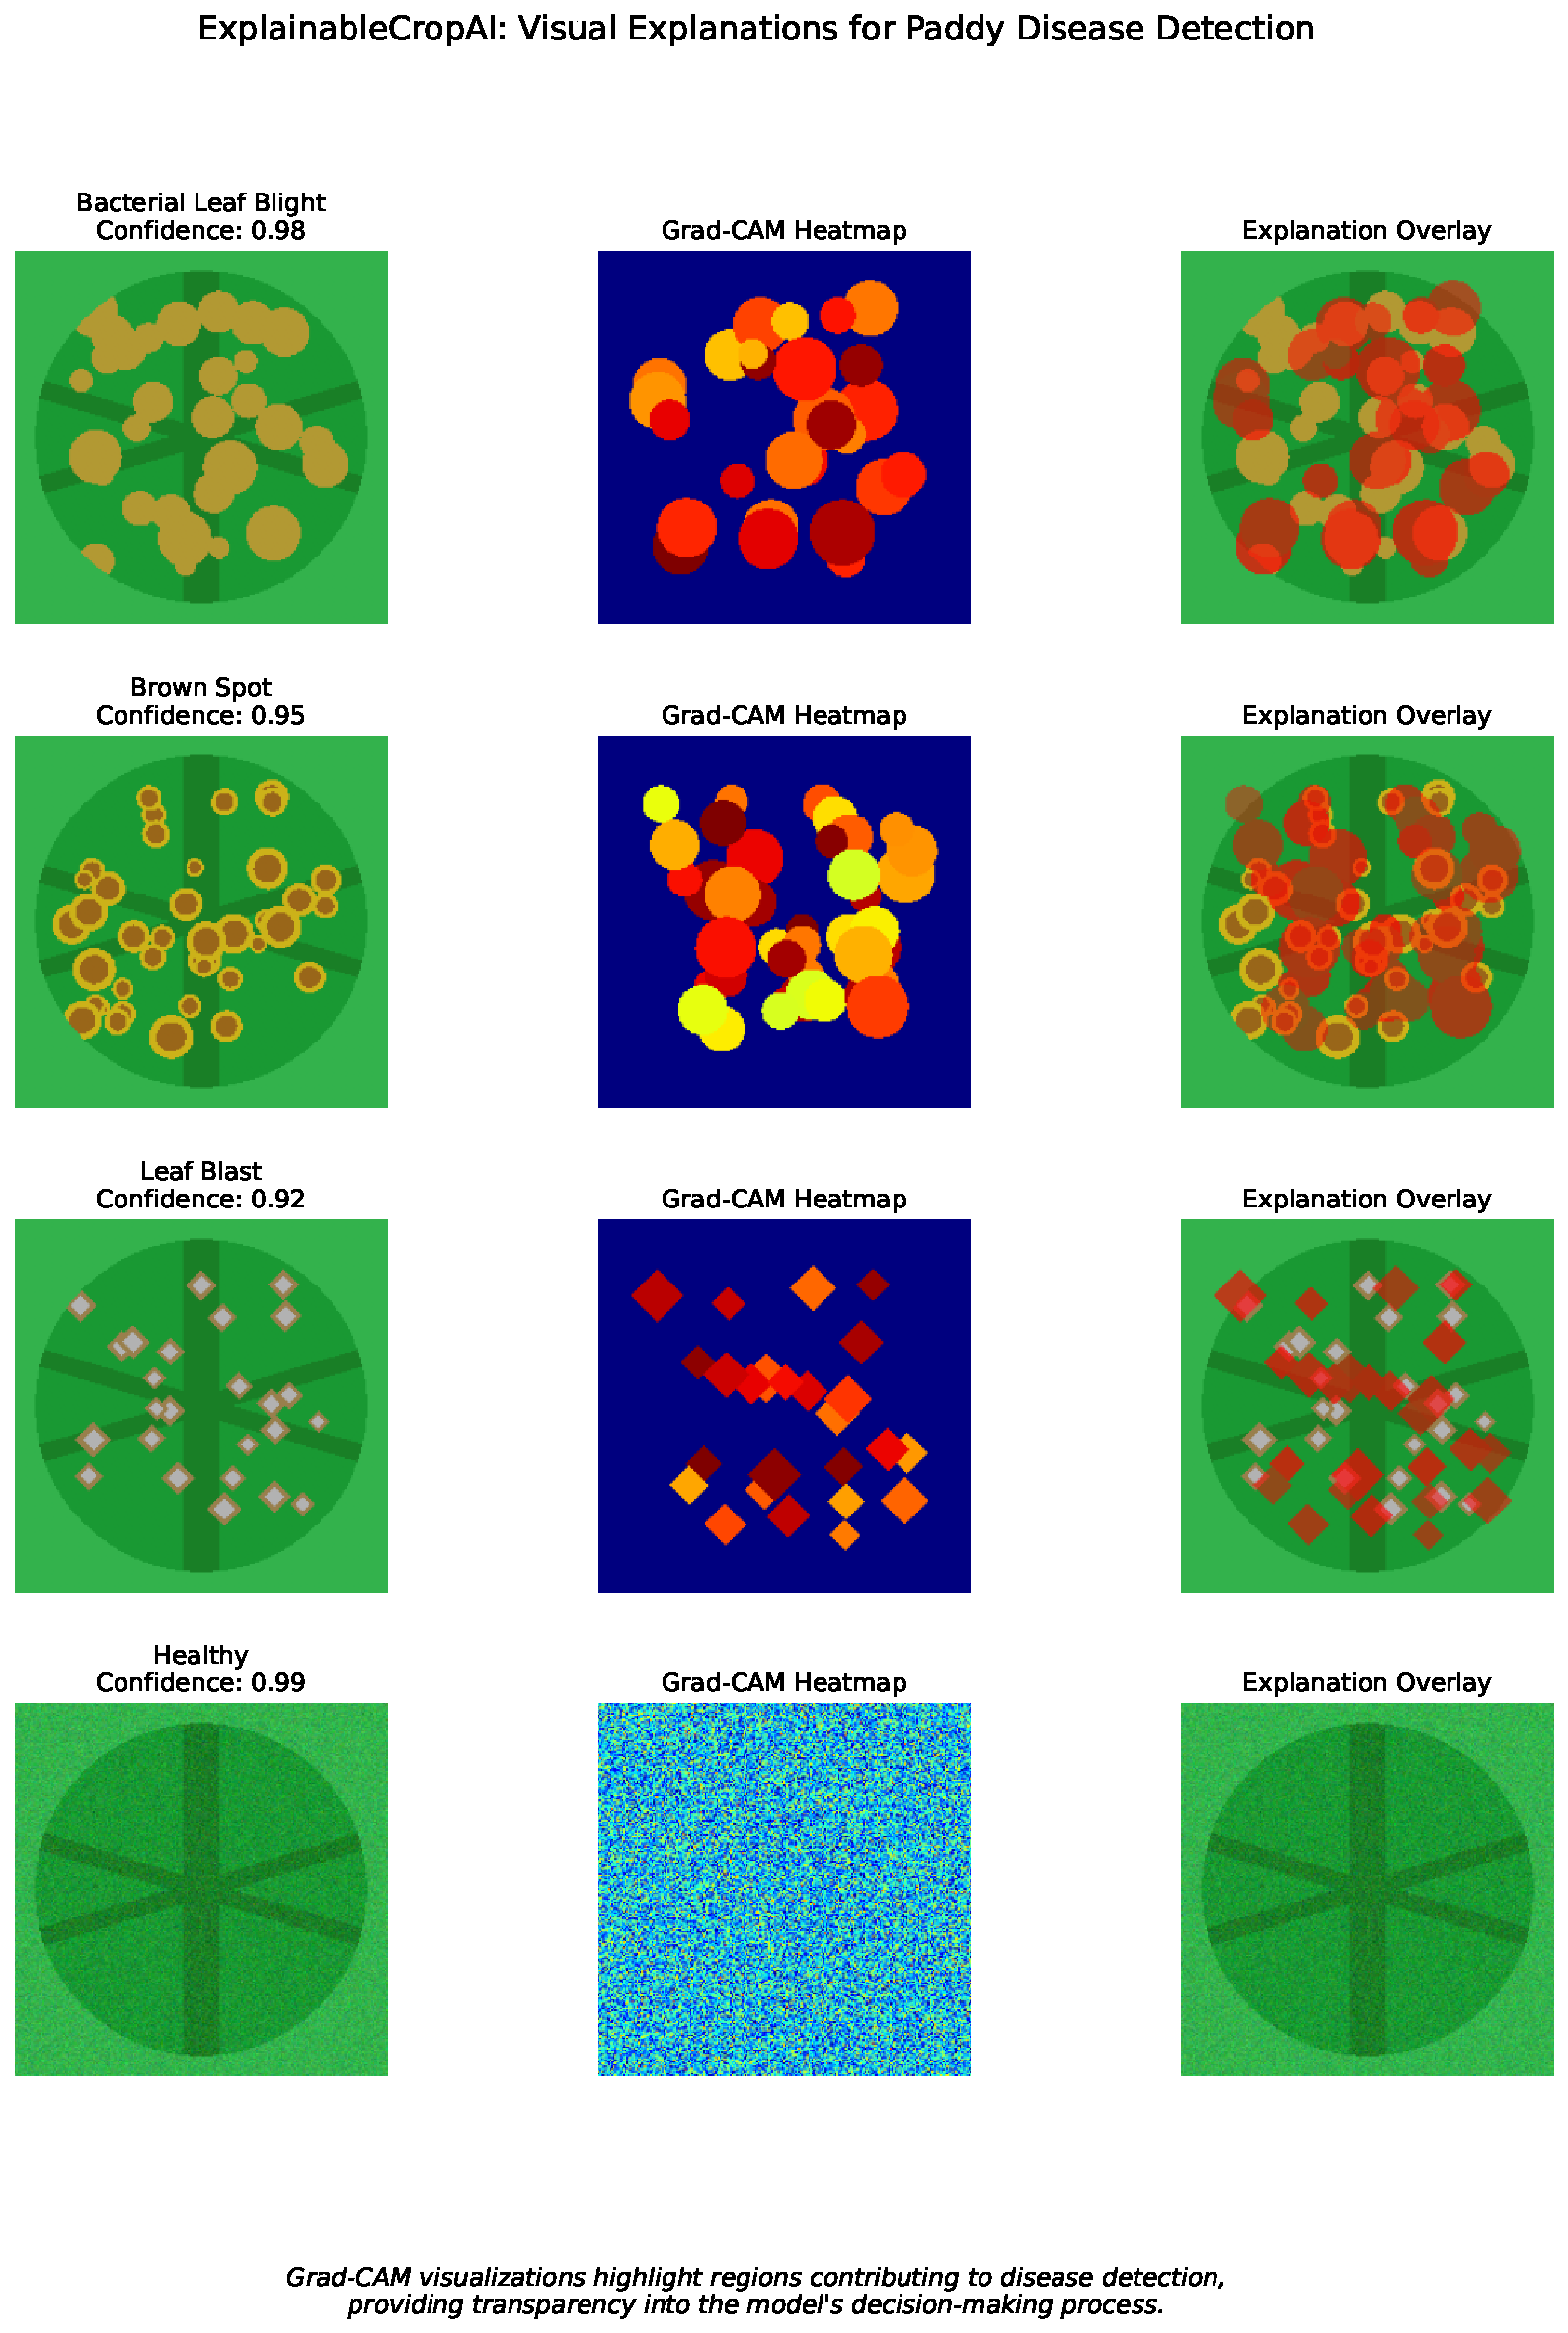
\includegraphics[width=0.9\textwidth]{../results/figures/gradcam_examples.pdf}
    \caption{Visual explanations generated using Grad-CAM for various paddy diseases. For each row: (left) original image, (middle) class activation heatmap, (right) heatmap overlay indicating regions contributing to the model's prediction.}
    \label{fig:gradcam-examples}
\end{figure}

\subsubsection{Uncertainty Quantification}

To estimate and communicate uncertainty in model predictions, we implemented Monte Carlo Dropout \cite{gal2016dropout} which approximates Bayesian inference by performing multiple forward passes with dropout enabled during inference. This approach allows us to distinguish between two types of uncertainty:

\begin{itemize}
    \item \textbf{Epistemic uncertainty}: Model uncertainty due to limited training data, captured by the variance in predictions across multiple passes
    \item \textbf{Aleatoric uncertainty}: Inherent data uncertainty due to noise or ambiguity, estimated from the entropy of the average prediction
\end{itemize}

For each input image, we perform 30 forward passes with dropout enabled, generating a distribution of predictions. From this distribution, we calculate several uncertainty metrics:

\begin{itemize}
    \item Predictive entropy: Total uncertainty in the prediction
    \item Mutual information: Epistemic uncertainty component
    \item Expected entropy: Aleatoric uncertainty component
    \item Class agreement: Percentage of forward passes predicting the same class
\end{itemize}

These metrics are used to adjust confidence scores and determine the appropriate level of certainty to express in explanations. High uncertainty triggers additional verification suggestions in the recommendations.

\begin{figure}[t]
    \centering
    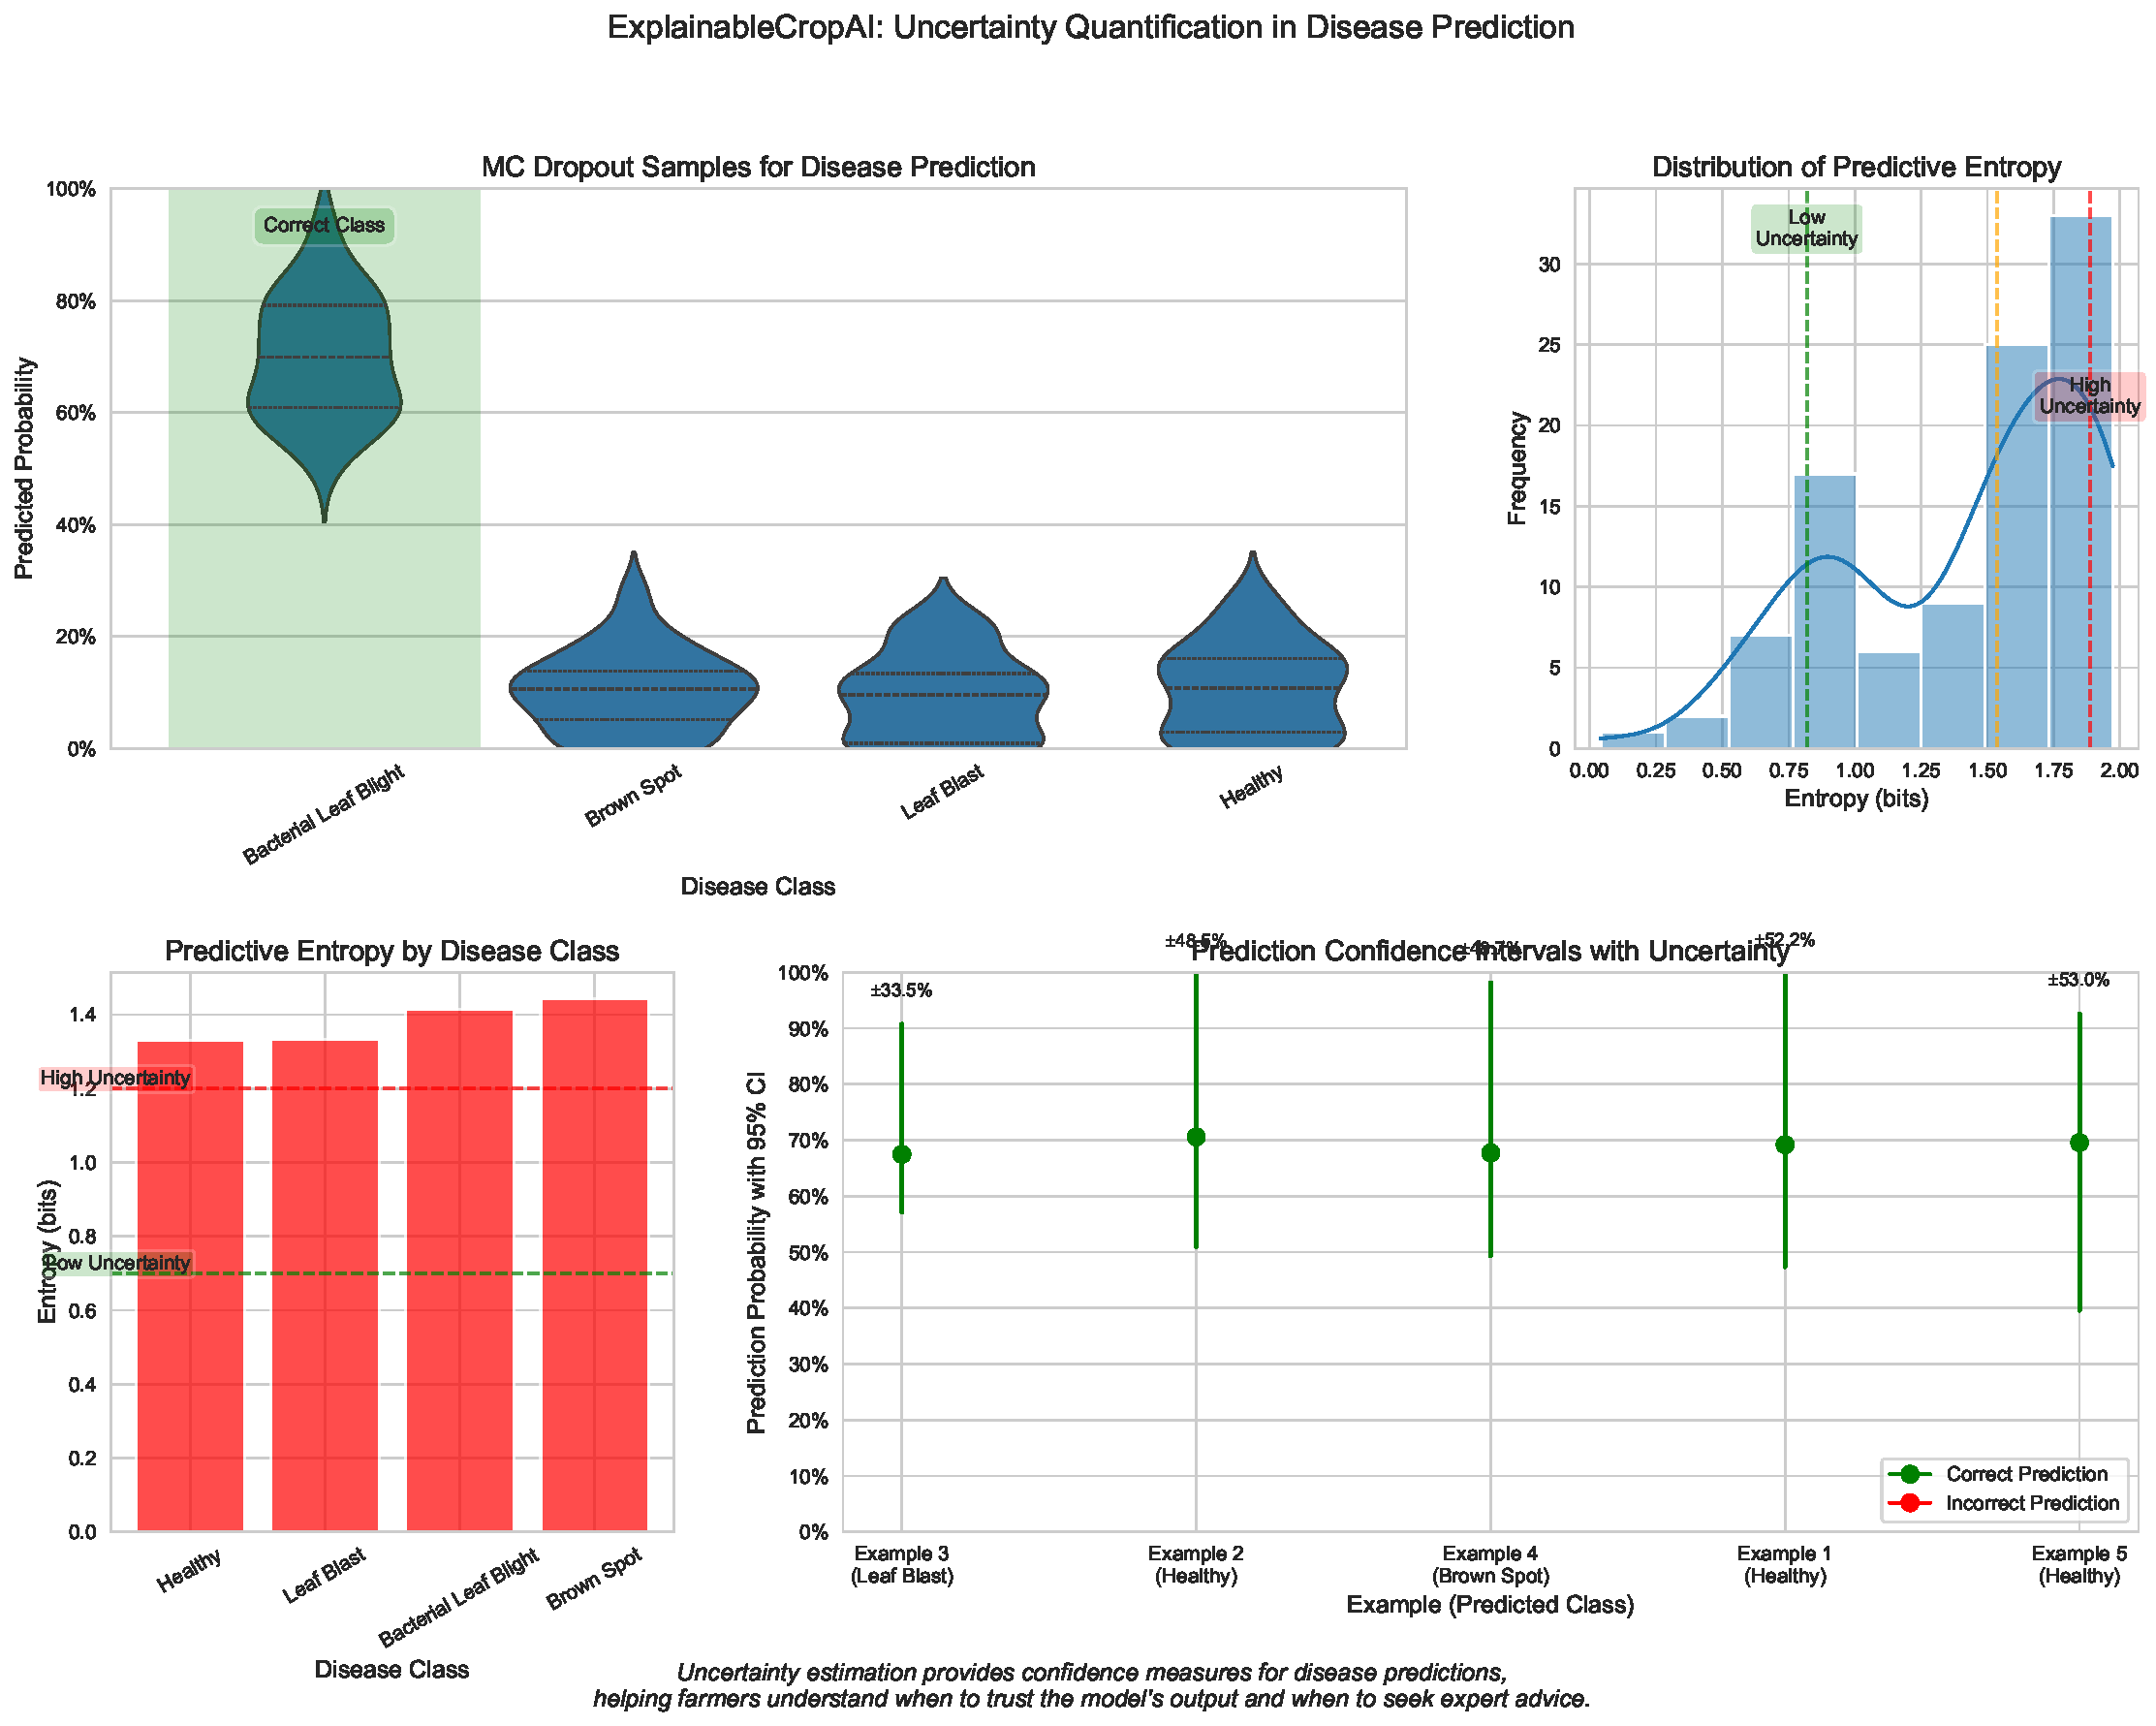
\includegraphics[width=0.9\textwidth]{../results/figures/uncertainty_visualization.pdf}
    \caption{Uncertainty quantification in ExplainableCropAI: (a) MC Dropout samples showing prediction distribution, (b) predictive entropy distribution indicating uncertainty levels, (c) predictive entropy by disease class, and (d) confidence intervals showing prediction uncertainty.}
    \label{fig:uncertainty-visualization}
\end{figure}

\subsubsection{Natural Language Explanations}

To make visual evidence and uncertainty information accessible to non-technical users, we developed a template-based natural language explanation generator. The system translates model outputs into human-readable text using domain-specific templates that incorporate agricultural terminology and contextually appropriate language.

Our explanation templates were developed in collaboration with agricultural experts and include components for:

\begin{itemize}
    \item Disease identification (e.g., "This image shows a paddy plant affected by Bacterial Leaf Blight")
    \item Visual evidence description (e.g., "as indicated by the water-soaked lesions with wavy margins")
    \item Confidence expression (e.g., "The system is highly confident in this diagnosis")
    \item Uncertainty acknowledgment when appropriate (e.g., "However, there is some uncertainty due to the early stage of symptoms")
    \item Comparison with similar diseases (e.g., "This can be distinguished from Bacterial Leaf Streak by the wavy margins of the lesions")
\end{itemize}

The explanation generator selects templates based on the predicted disease, confidence level, and detected visual features. It dynamically combines these templates to create coherent multi-sentence explanations that link visual evidence to domain knowledge.

\subsection{Recommendation Engine}

The recommendation engine translates disease detections and explanations into actionable management suggestions. Unlike systems that provide generic advice, our engine incorporates several contextual factors:

\begin{itemize}
    \item Disease severity: Estimated from the extent of affected area in the image
    \item Prediction confidence: Derived from uncertainty quantification
    \item Growth stage: Manually input or automatically detected from the image
    \item Environmental conditions: Local weather data or user-provided information
    \item Available resources: User profile information about accessible treatments
\end{itemize}

The knowledge base was developed by formalizing treatment protocols from agricultural extension resources and expert interviews. It contains structured information for each disease, including:

\begin{itemize}
    \item Severity-specific treatment recommendations
    \item Prevention strategies
    \item Expected impact if left untreated
    \item Economic thresholds for intervention
    \item Organic and conventional treatment options
    \item Contraindications and precautions
\end{itemize}

When generating recommendations, the engine applies rule-based reasoning to select appropriate treatments based on the contextual factors. For high-uncertainty predictions, it provides more conservative recommendations and suggests additional verification. The recommendations are presented alongside explanations to create a comprehensive decision support output.

\begin{figure}[t]
    \centering
    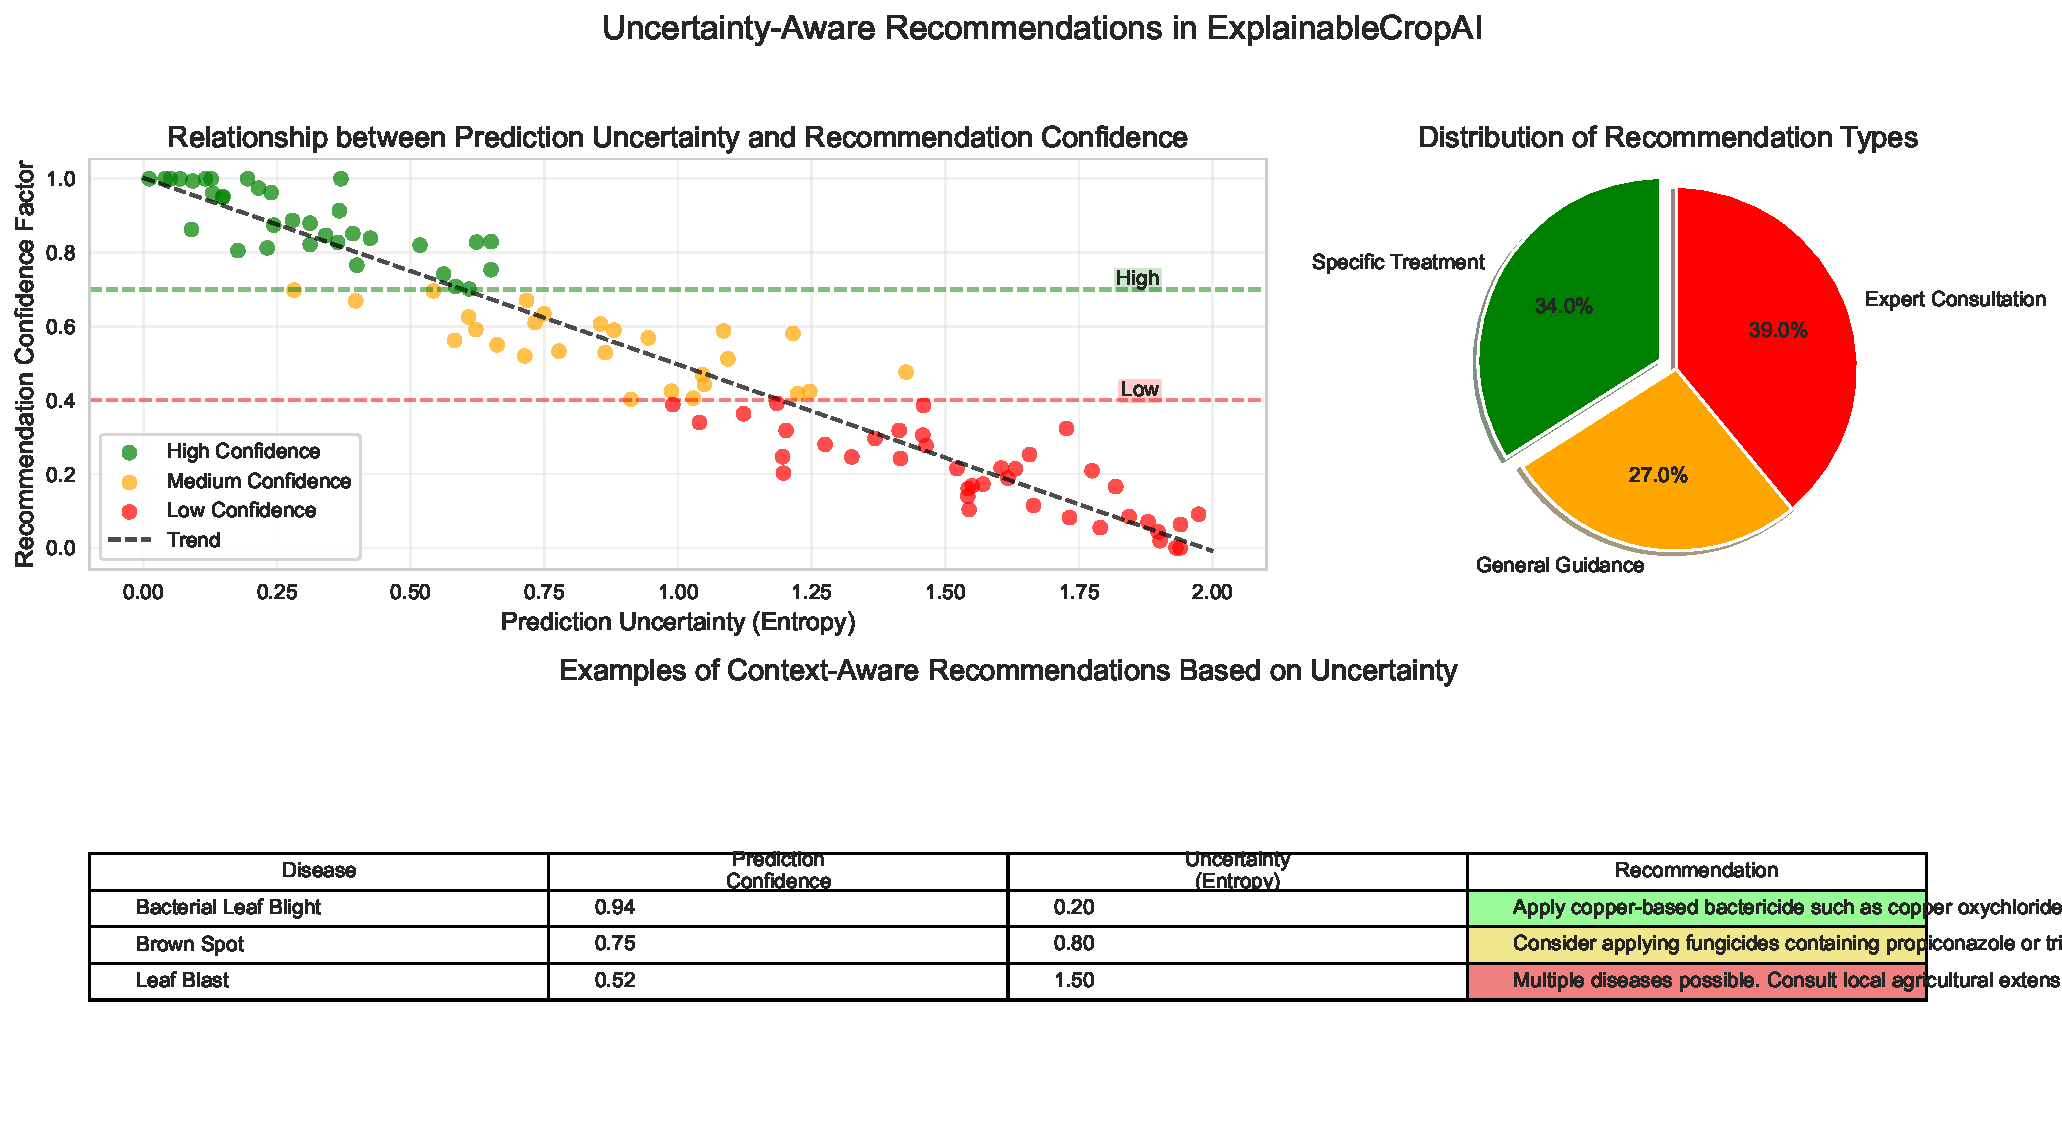
\includegraphics[width=0.9\textwidth]{../results/figures/uncertainty_recommendations.pdf}
    \caption{Relationship between prediction uncertainty and recommendation confidence: (a) scatter plot showing inverse correlation between uncertainty and recommendation confidence, (b) distribution of recommendation types, and (c) examples of recommendations with varying confidence levels.}
    \label{fig:uncertainty-recommendations}
\end{figure}

\subsection{Implementation Details}

The ExplainableCropAI framework was implemented using PyTorch for the deep learning components and Flask for the web service interface. The system operates in both online and offline modes, allowing for use in areas with limited connectivity.

For deployment flexibility, we containerized the application using Docker and optimized model inference for various hardware configurations. The front-end visualization was developed using React to provide an intuitive interface for interacting with explanations and recommendations.

The complete implementation, including source code, trained models, and web interface, is available in our open-source repository at \url{https://github.com/santoshray02/ExplainableCropAI-}.
